{\chapter{Analyse}}
\label{sec:analyse}
Zusätzlich zu den maschinellen Lernkomponenten liefert Unity auch Demonstrationsumgebungen, in denen verschiedene Lösungen für gängige Verstärkungslernprobleme implementiert sind. In der Walker-Demo wird ein physisch simulierter Charakter darauf trainiert, zu einem Zielwürfel zu laufen. Diese Demo-Umgebung implementiert bereits einige Grundlagen für die Steuerung eines physisch simulierten Charakters. Aus diesem Grund wird in dieser Arbeit die Walker-Demo als Grundlage für die Entwicklung genutzt. In diesem Kapitel wird daher die Walker-Demo analysiert, um in den folgenden Kapiteln darauf aufzubauen.

\section{Szenenaufbau}

\begin{figure}[H]
  \centering  
  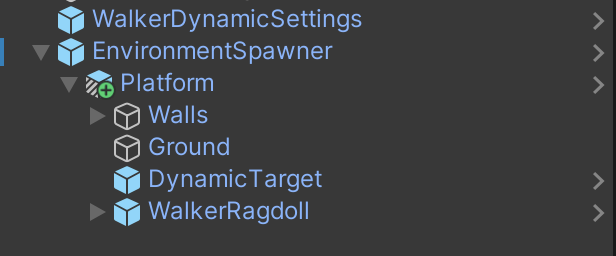
\includegraphics[scale=0.8]{img/walker_demo_hierarchy.png}
  \caption{Walker-Demo Hierarchy}
  \label{fig:walker_demo_hierarchy}
\end{figure}

\begin{figure}[H]
  \centering  
  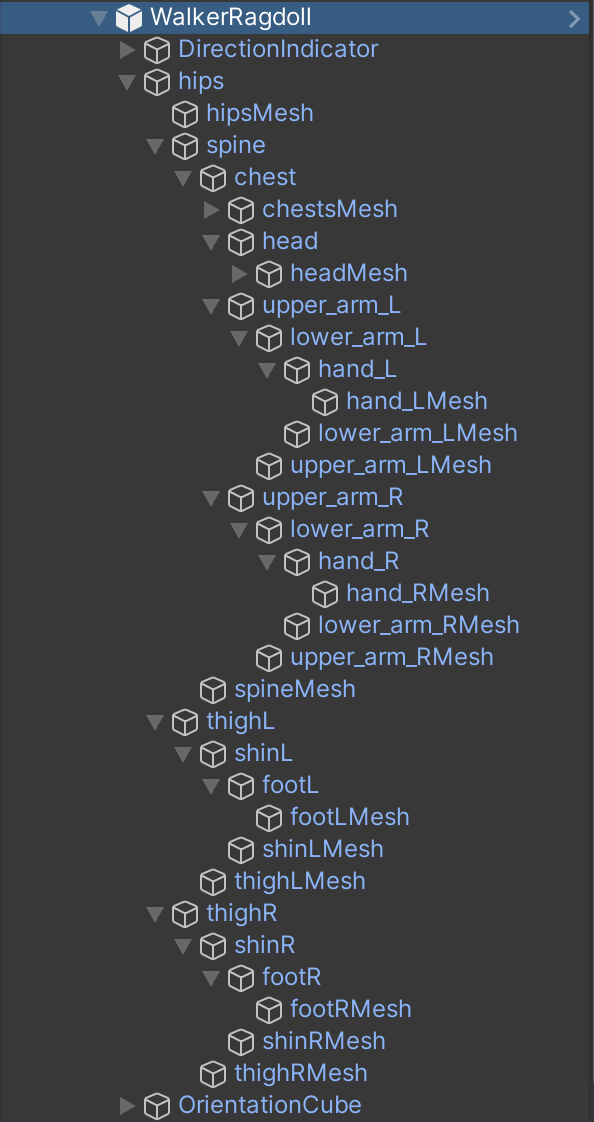
\includegraphics[scale=0.5]{img/agent_hierarchy.png}
  \caption{Agent Hierarchy}
  \label{fig:agent_hierarchy}
\end{figure}


\section{Physikkomponenten und -konfiguration}
Der Körper besteht aus 11 Kapseln, drei Kugeln und 2 Quadern, jeder dieser Formen hat eine Festkörper und eine Kollisions Physikkomponente. Zwischen den Körperteilen werden die Gelenke als Kugelgelenke simuliert.

\begin{center}
{\rowcolors{2}{lightgray}{gray!50!lightgray!50}
\begin{tabular}{ |p{3cm}|p{3cm}|p{2cm}|p{4cm}|p{2cm}| }
\hline
Körperteil& Verbundenes Körperteil & Gewicht & Winkellimits & Form \\
\hline
Hüfte & - & 15kg & - & Kapsel \\
Wirbelsäule & Hüfte & 10kg & x(-20,20) y(-20,20) z(-15,15) & Kapsel \\
Oberkörper & Wirbelsäule & 8kg & x(-20,20) y(-20,20) z(-15,15) & Kapsel \\
Kopf & Oberkörper & 6kg & x(-30,10) y(-20,20) & Kugel \\
Oberarm LR & Oberkörper & je 4kg & x(-60,120) y(-100,100) & Kapsel \\
Unterarm LR & Oberarm & je 3kg & x(0,160) & Kapsel \\
Hand LR & Unterarm & je 2kg & - & Kugel \\
Oberschenkel LR & Hüfte & je 14kg& x(-90,60) y(-40,40) & Kapsel \\
Unterschenkel LR & Oberschenkel & je 7kg &  x(0,120) & Kapsel \\
Fuß LR & Unterschenkel & je 5kg & x(-20,20 y(-20,20) z(-20,20) & Quader \\
\hline
\end{tabular}}
\end{center}

\section{Agent implementierung}
lernablauf (Beobachtung, Aktionen ausführen, Belohnungsfunktion, einrichtung)

\begin{figure}[H]
  \centering  
  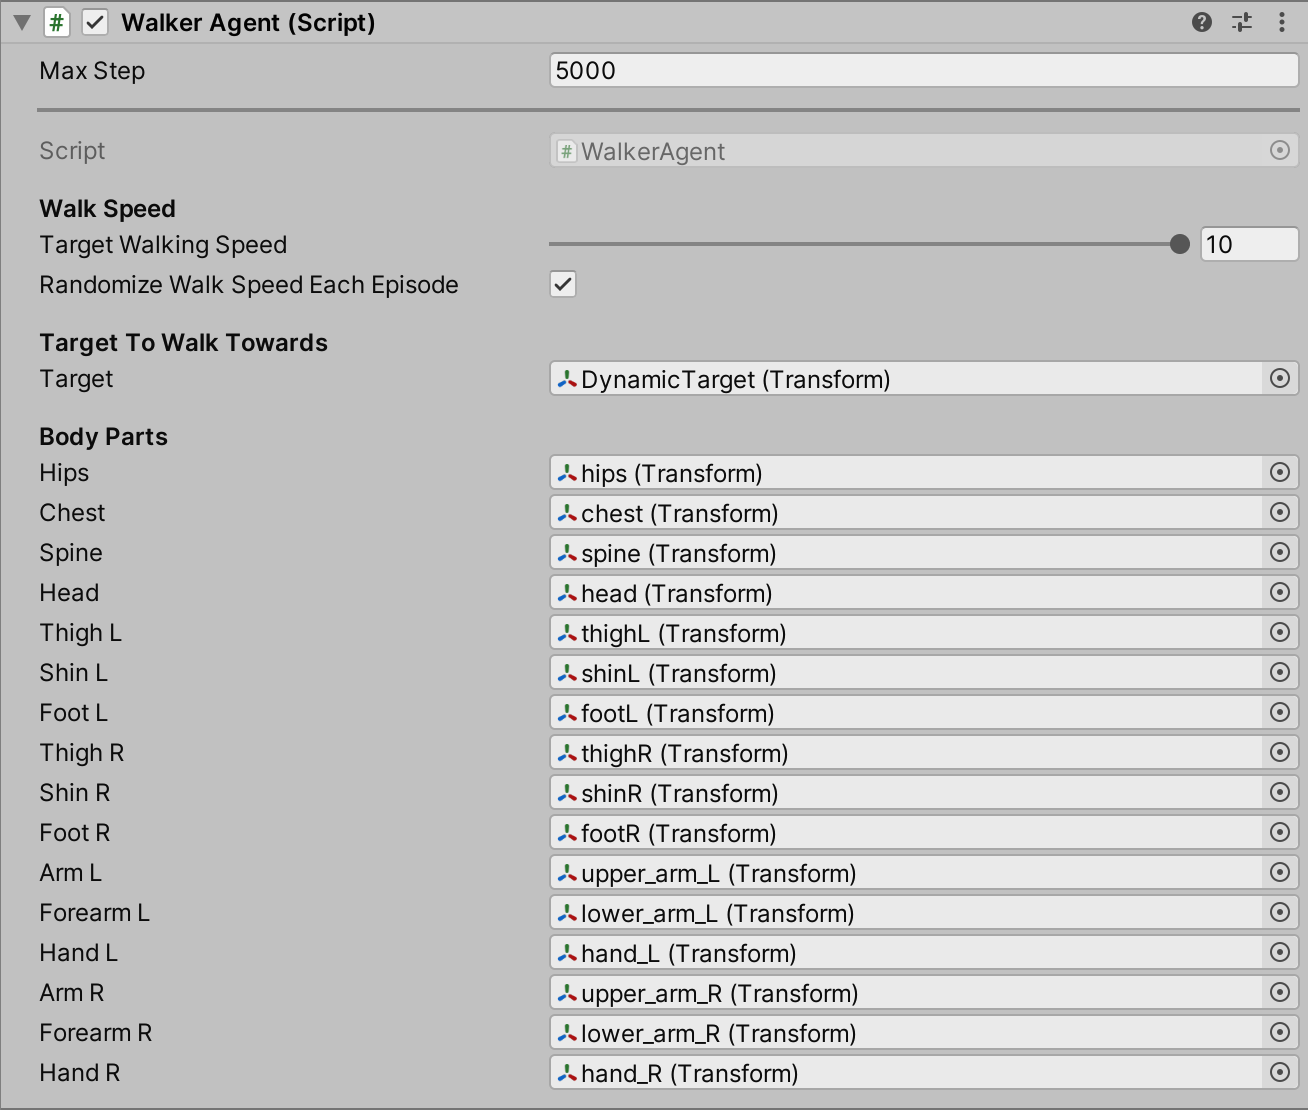
\includegraphics[scale=0.5]{img/agent_konfiguration.png}
  \caption{Agent Konfiguration}
  \label{fig:agent_konfiguration}
\end{figure}

Agent Code hier einfügen? oder evtl. im Anhang?

\section{Ziel}
Ziele (target controller)